\documentclass[a4paper, 12pt]{article}
\usepackage[top=2cm, bottom=2cm, left=2.5cm, right=2.5cm]{geometry}
\usepackage[utf8]{inputenc}
\usepackage[portuguese]{babel}
\usepackage{indentfirst}
\usepackage{graphicx}
\usepackage{float}

\usepackage{subcaption}


\title{Modelos matemáticos para identificar o perfil 3d de superfícies digitalizados por meio da visão monocular com projeção de luz estruturada}
\author{Elisângela Ribeiro, Fernando Pujaico Rivera, Bianca Batista Barreto,\\Roberto Alves Braga Junior, Marco Antônio Barbosa 
\\elismar1952@hotmail.com; fernando.pujaico.rivera@gmail.com;
\\biabarreto89@gmail.com; robbraga@gmail.com; marco.fisioedu@ufla.br}


\begin{document}
\maketitle

\section*{Resumo}
Uma imagem é a representação visual de um objeto real em uma superfície sensível gerada a partir de um foco central. Esta pode variar de acordo com os dados intrínsecos da câmera e da geometria da cena. Sendo a luz estruturada um processo de projetar um padrão conhecido em uma cena, a forma como o padrão se deforma quando atinge a superfície permite que sistemas de visão calculem a profundidade e informações das superfícies dos objetos na cena. Partindo desse pressuposto, este trabalho tem o objetivo de identificar o perfil de um objeto em um plano de referência, a partir de dados intrínsecos da câmera, da geometria da cena e da luz estruturada, por meio de visão monocular. Para isso foi desenvolvido uma função de correção envolvendo modelos matemáticos para identificar todos os parâmetros que compõem o sistema gerador da imagem. Esse sistema é composto pelas variáveis de entrada de acordo com a configuração experimental. Os resultados mostraram que foi possível identificar as distorções dos eixos X, Y e Z e traçar o perfil do objeto em análise em três dimensões.


\textbf{Palavra-chave:}  Luz estruturada; perfil; três dimensões.

\section*{Abstract}

An image is the visual representation of a real object on a sensitive surface generated from a central focus. This can vary according to the intrinsic data of the camera and scene geometry. Being structured light is a process of projecting a known pattern in a scene, the way the pattern deforms when it reaches the surface allows vision systems to calculate the depth and information of the surfaces of objects in the scene. Based on this assumption, this work aims to identify the profile of an object in a reference plane, using intrinsic data from the camera, the geometry of the scene and structured light, through monocular vision.For this purpose, a correction function was developed involving mathematical models to identify all the parameters that make up the image generating system. This system is composed of the input variables according to the experimental configuration. The results showed that it was possible to identify the distortions of the X, Y and Z axes and to profile the object under analysis in three dimensions.

\textbf{Keywords:}Structured light; profile; three dimensions. 



\section{Introdução}

Aqui vem o texto



\section{Material e Métodos}

Os procedimentos metodológicos para a execução do projeto seguiram os seguintes passos:

• Montagem da configuração experimental;

• Digitalização de superfície conhecida;

• Binarização de uma imagem em cores;

• Otimizando experimentalmente os valores dos parâmetros. 

Todos os experimentos foram realizados nas dependências da Universidade Federal de Lavras (UFLA), dividido entre os laboratórios nº 2 e 7 do Centro de Desenvolvimento à Instrumentação aplicado à Agropecuária (CEDIA), ligado ao Departamento de Automática.

A configuração experimental foi elaborada por meio da visão monocular (RIBEIRO, 2014) com projeção de Luz estruturada para a digitalização de várias superfícies.

Nessa configuração, com o auxílio do projetor conectado ao computador, projetam-se linhas horizontais sobre o objeto em análise, de forma a identificar o delineamento da superfície.


\subsection{Montagem da configuração experimental}

Para a configuração do sistema, utilizou-se de uma fonte de luz como o projetor e apenas uma câmera, ambos dispostos em ângulos em relação ao objeto, ilustrado na Figura \ref{arranjo-experimetal}, conhecido também como Luz estruturada (projeção de um padrão conhecido – como linhas horizontais que ao tocar o objeto desenha a sua superfície) por meio da visão monocular (utiliza apenas uma câmera).

\begin{figure}[H]
\centering
    \begin{subfigure}{.695\textwidth}
      \centering
      % include first image
      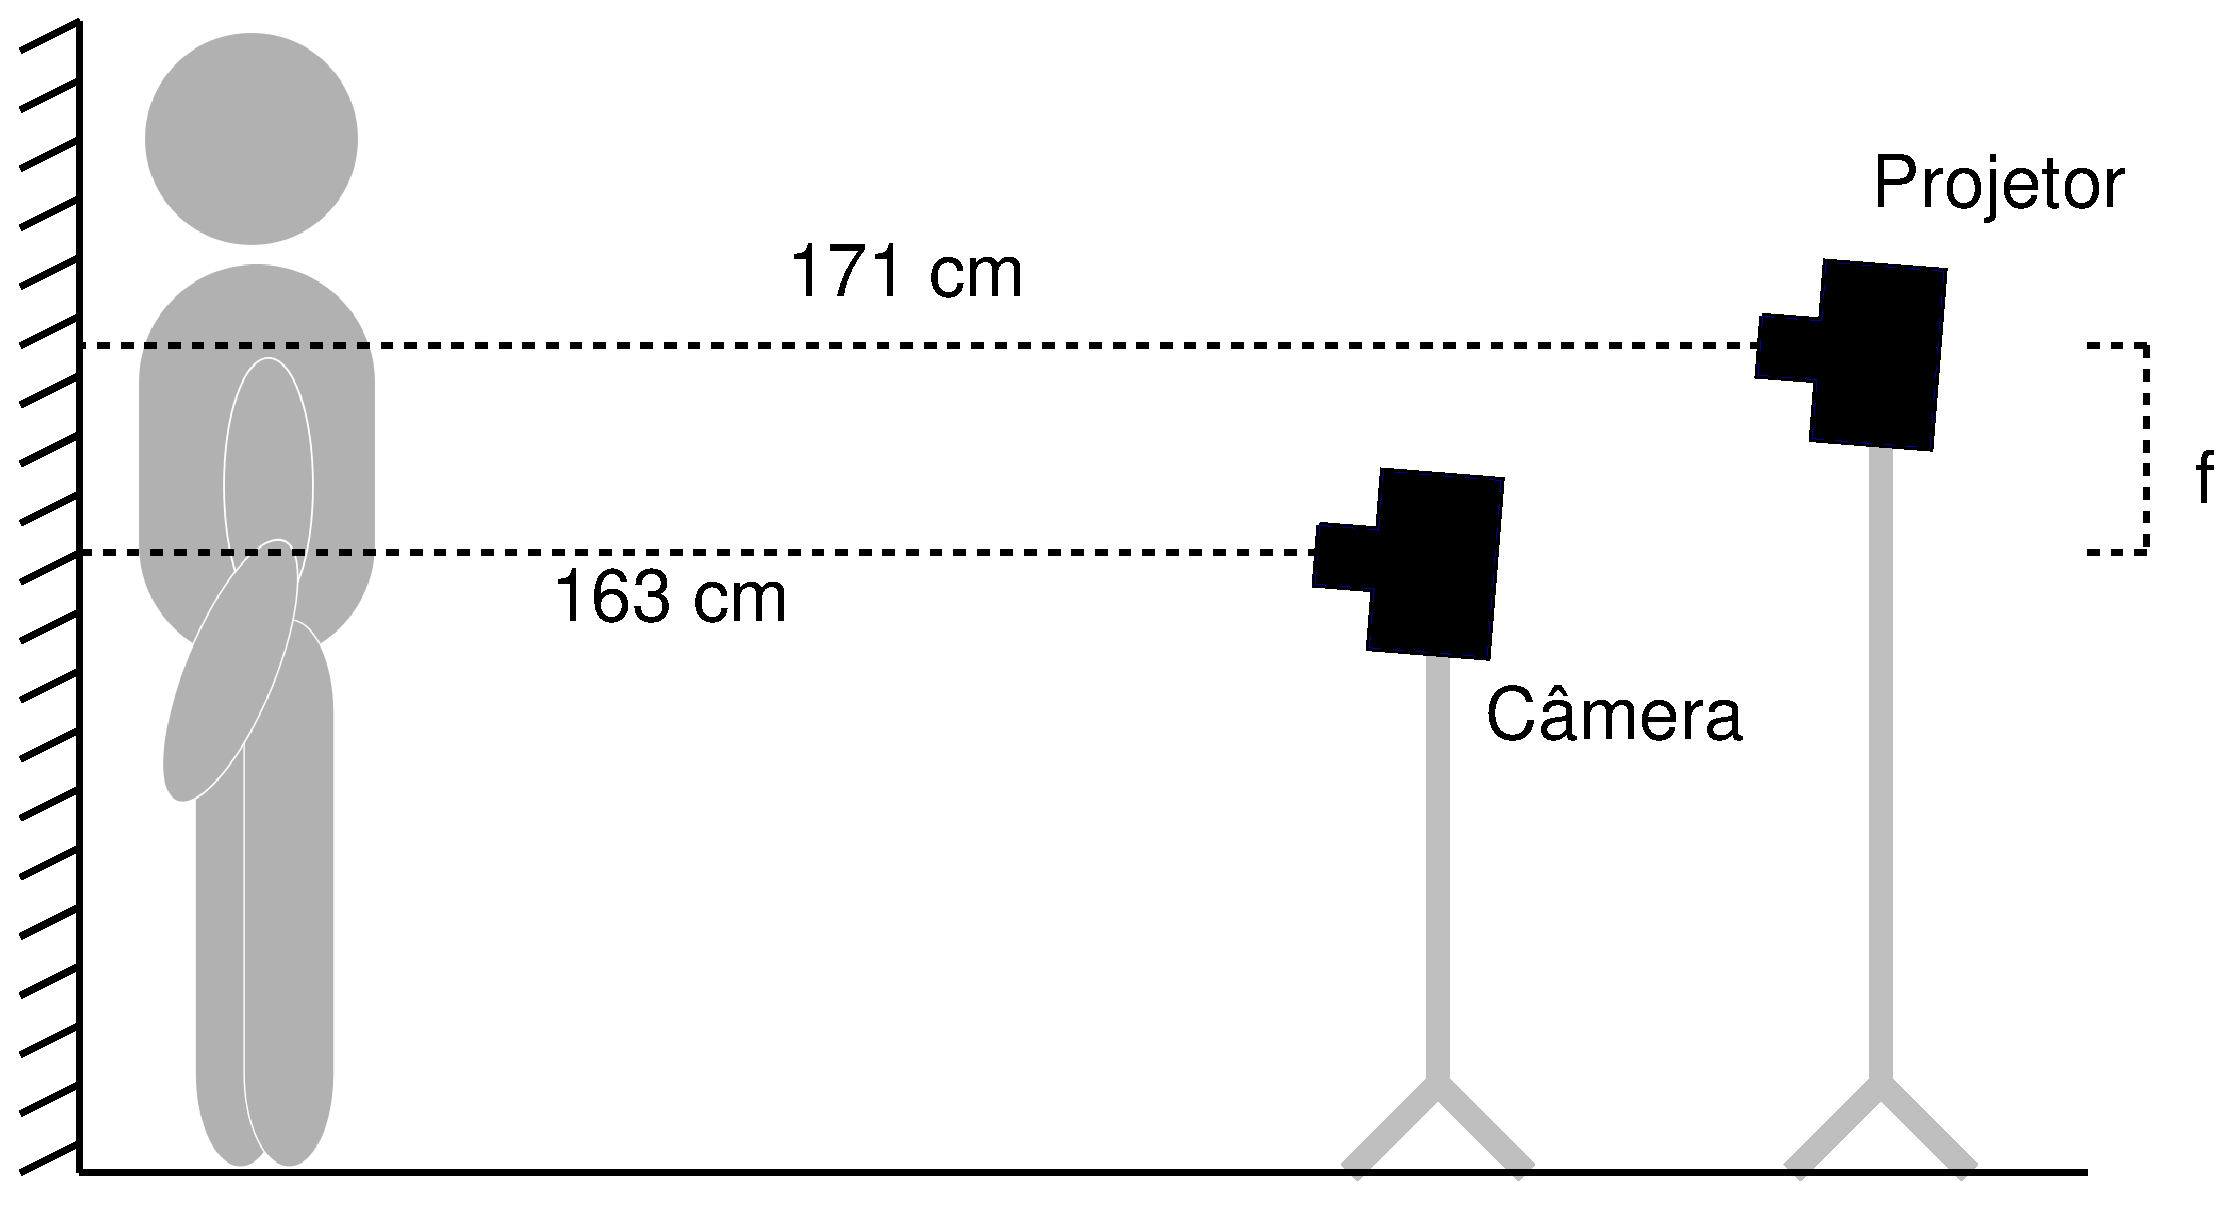
\includegraphics[width=.95\linewidth]{configuracao_sistema_1.eps}  
      \caption{Disposição do arranjo experimental}
      \label{arranjo-experimetal:1}
    \end{subfigure}
    \begin{subfigure}{.295\textwidth}
      \centering
      % include first image
      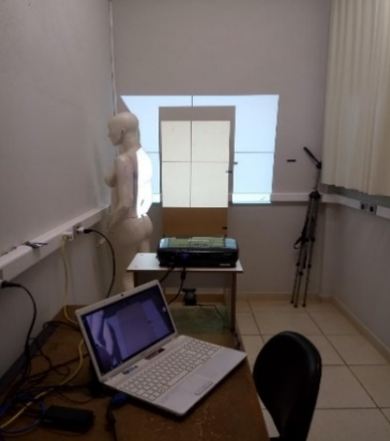
\includegraphics[width=.95\linewidth]{configuracao_sistema_2.png}
      \caption{Fotografia do arranjo experimental}
      \label{arranjo-experimetal:2}
    \end{subfigure}	
\caption{Arranjo experimental utilizando luz estruturada}
\label{arranjo-experimetal}
\end{figure}


Os equipamentos utilizados na configuração experimental foram: uma webcam com as seguintes configurações: Hd, 3.0 Mb, Usb da marca Logitech C270 960-000691, um projetor multimídia Benq com as seguintes descrições: Mx525b 3200 Lumens/Xga/Hdmi/3D Ready/Bndes e um computador portátil Sony Vaio Core i3. 

Na configuração, a fonte de luz ficou fixada a uma distância de 171 cm do objeto. A câmera ficou fixada a uma distância de 136 cm do objeto, conforme ilustra a Figura \ref{arranjo-experimetal}.  Com a utilização de um computador portátil conectado ao projetor, projetaram linhas sobre o objeto.

Ao montar a configuração experimental utilizando visão monocular, foi possível identificar várias variáveis no setup, conforme ilustra a Figura \ref{setup com as variaveis} a seguir.

\begin{figure}[H]
	\centering
		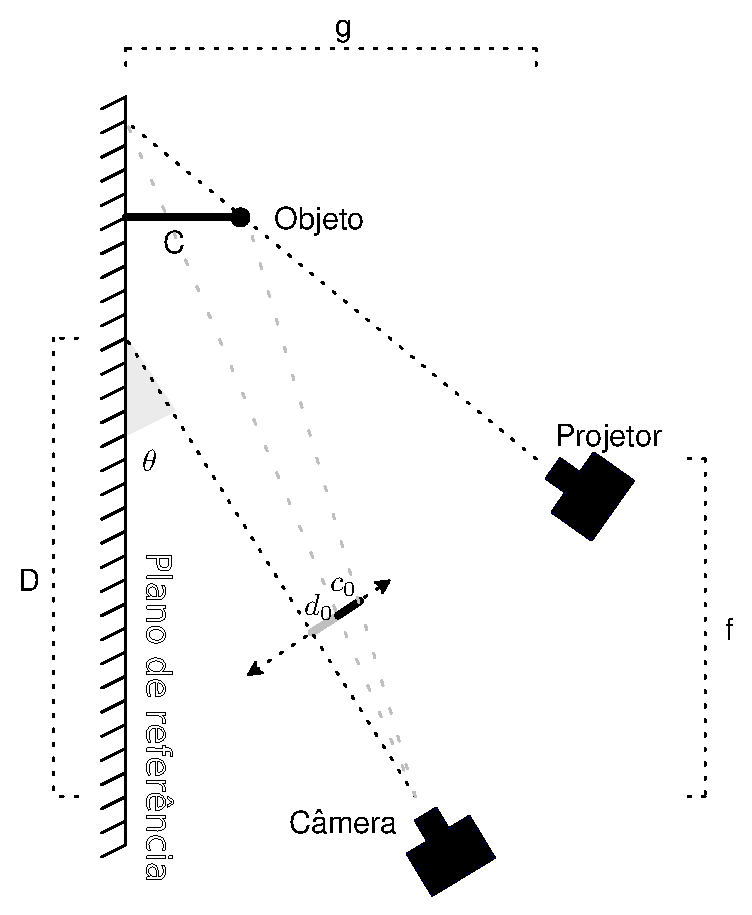
\includegraphics[width=.55\linewidth]{vista_sagital.eps}
	\caption{Variáveis da Configuração Experimental em uma vista sagital}
	\label{setup com as variaveis}
\end{figure}

Sendo:

g: Medida em centímetros da altura do projetor em relação ao plano de referência;

f:  Distância em centímetros entre o projetor e a câmera;	          

Q: Ângulo formado entre a câmera e o plano de referência;

$h_0$: Distância focal em pixels da câmera em relação ao objeto;  

D:  Distância em centímetros entre sigma e beta;

C: Altura real do objeto, também identificado pela variável z;

$c_0$: Altura relativa em pixels do objeto na imagem digitalizada;

$d_0$: Diferença em pixels entre o ponto central real da imagem até a linha de referência projetada, sendo que esses dados estão em referência na fotografia digitalizada. 
 
Todas essas variáveis foram importantes para o desenvolvimento de modelos matemáticos utilizados nos algoritmos desenvolvidos. 

\subsection{Digitalização de uma superfície}

Com a câmera fixada em um tripé, capturou-se uma foto da projeção da linha sobre o objeto, conforme ilustra a Figura \ref{imagem_projecao_colorida}a. Em seguida, removeu-se o objeto, e o mesmo procedimento foi repetido para a captura da imagem do plano, conhecida como imagem referência ilustrado na Figura \ref{imagem_projecao_colorida}b. 

\begin{figure}[H]
	\centering
		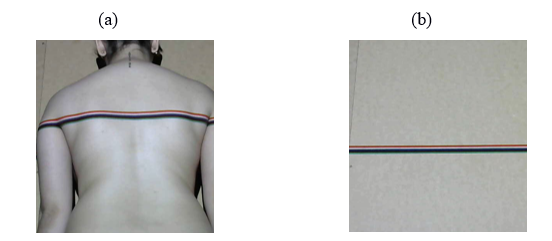
\includegraphics[width=.55\linewidth]{imagem_projecao_colorida.png}
	\caption{a- Imagem objeto b- Imagem referência}
	\label{imagem_projecao_colorida}
\end{figure}

As linhas projetadas nas costas dos humanos foram coloridas seguindo o padrão RGB (LUKAC; PLATANIOTIS, 2005) associado às cores preta e branca, de forma que uma das cinco cores projetadas fossem visualizadas nas fotos capturadas, pois o conjunto de amostras possuíam uma variedade de tonalidade na cor da pele.

No fluxograma da Figura \ref{fluxograma_identificar_3D}, é responsável pelo procedimento de transformação da imagem obtida na configuração em 3D, o qual primeiramente teve como objetivo apresentar o processo de transformação da imagem digitalizada, na configuração experimental, a uma representação em 3D. Para isso, foi necessário a captura das imagens objeto e referência com a projeção das linhas coloridas sobre as costas humana. Em seguida, foi desenvolvido um algoritmo para a binarização de uma imagem em cores.

\begin{figure}[H]
	\centering
		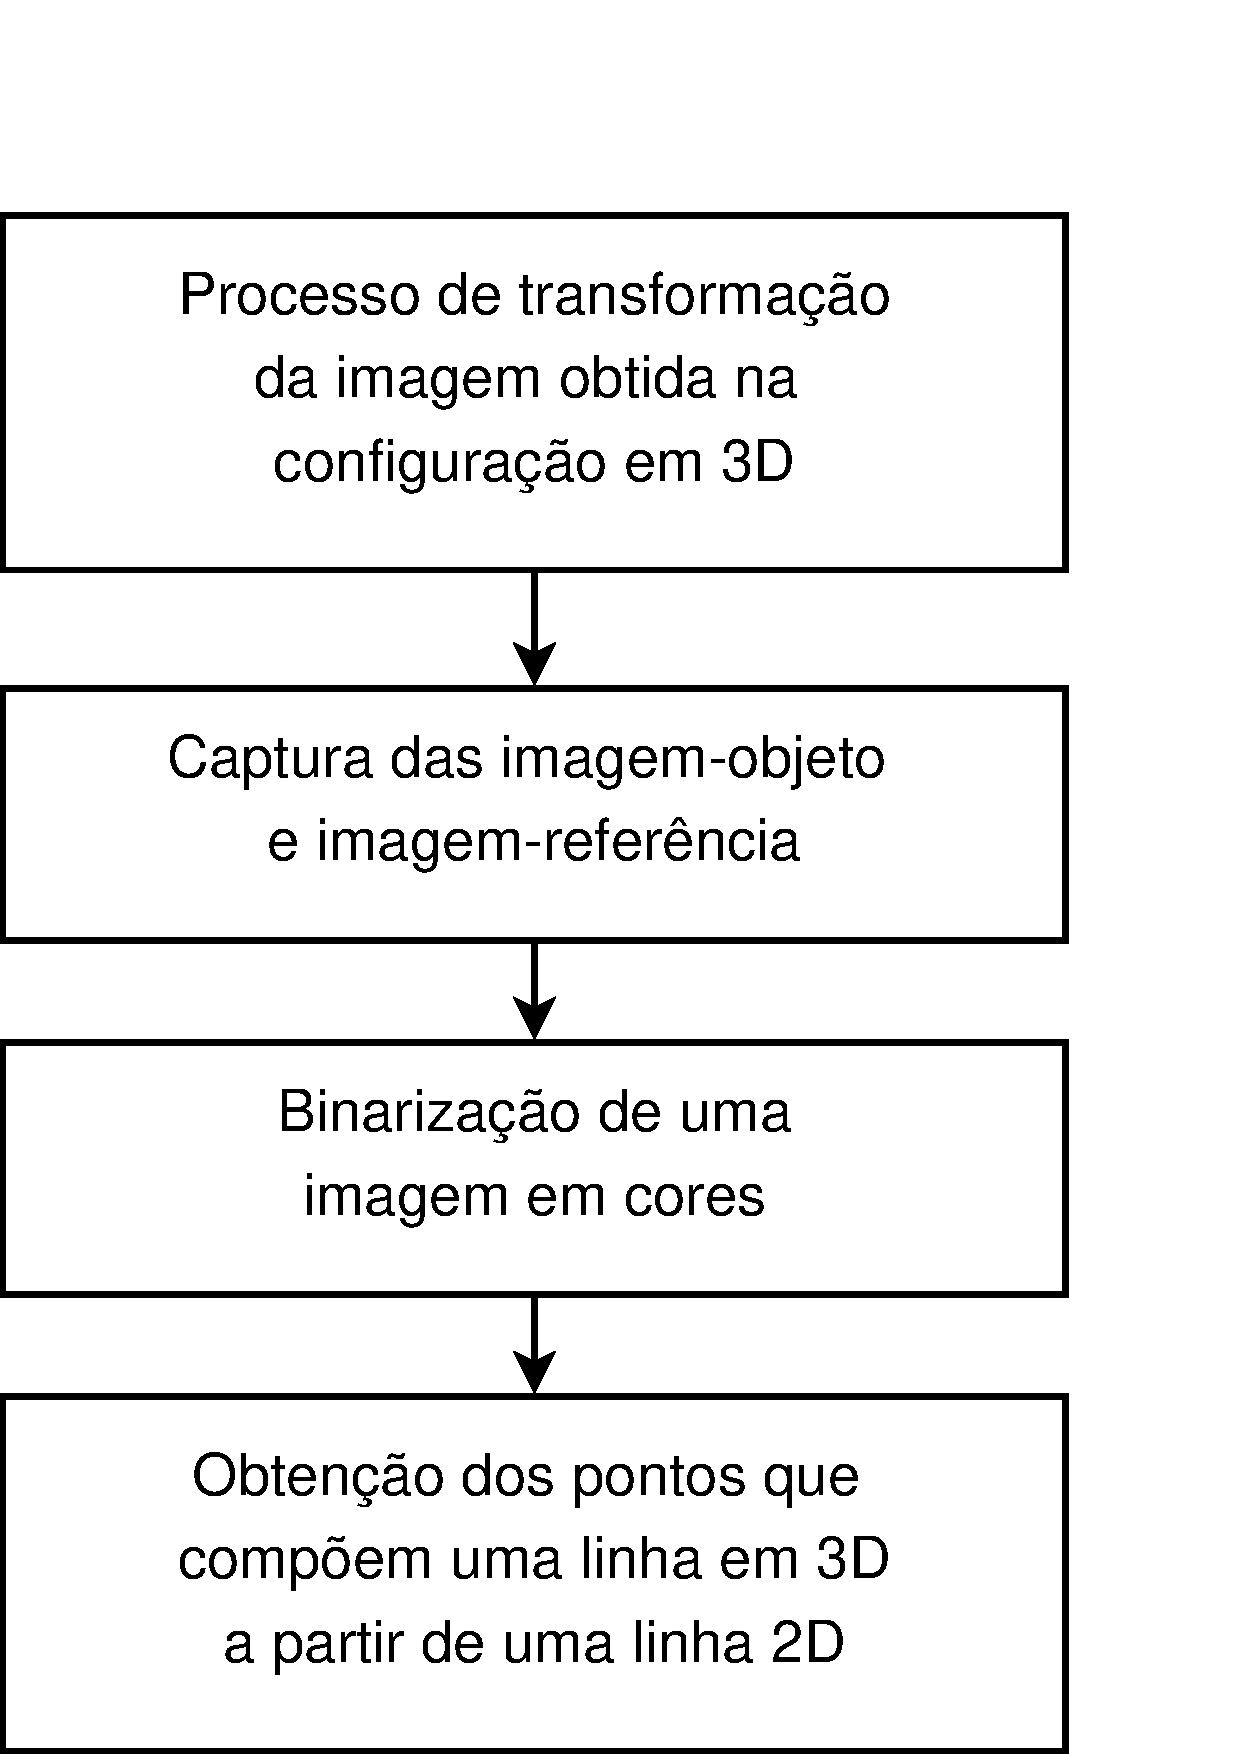
\includegraphics[width=.55\linewidth]{fluxograma_identificar_3D.png}
	\caption{Fluxograma para identificar o perfil 3D}
	\label{fluxograma_identificar_3D}
\end{figure}

\subsection{Binarização de uma imagem em cores}

Esta Seção foi responsável por transformar as imagens capturadas em apenas linhas (binária), ou seja, deixar em evidência binária somente a linha de melhor delineamento, que no caso das imagens digitalizadas, a cor vermelha foi a que teve o melhor destaque nas costas dos indivíduos.

Para realizar esse processo, um algoritmo baseado em identificação de cores foi desenvolvido. Ele teve como dados de entrada a imagem original digitalizada, na qual o algoritmo percorreu toda ela e identificou a cor desejada e descartou todos as outras, obtendo, assim, como imagem final somente a linha da superfície digitalizada, conforme ilustra a Figura \ref{identificar linha na imagem}.

\begin{figure}[H]
	\centering
		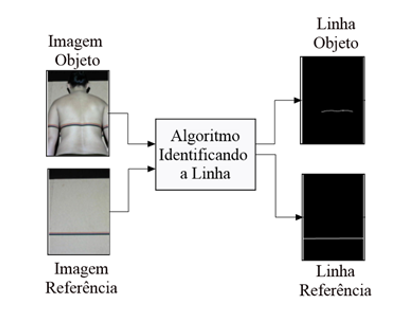
\includegraphics[width=.55\linewidth]{identificar_linha_imagem.png}
	\caption{Processo para identificação da linha na imagem digitalizada}
	\label{identificar linha na imagem}
\end{figure}

\subsection{Lógica matemática para detectar as cores}

Inserir o texto com as formulas do arquivo enviado


\section{Otimizando experimentalmente os valores dos parâmetros}
Nesta Seção, foi desenvolvido o sistema representado na Figura \ref{sitema_otimizacao}, o qual foi composto por cinco variáveis ($h_0$, D, Q, f e g), e seus parâmetros foram possíveis de serem identificados de forma manual que, eventualmente, possui erro devido à imprecisão de medição humana. Porém, é necessário que esses parâmetros sejam o mais real possível, sendo necessário realizar uma aproximação desses dados.

\begin{figure}[H]
	\centering
		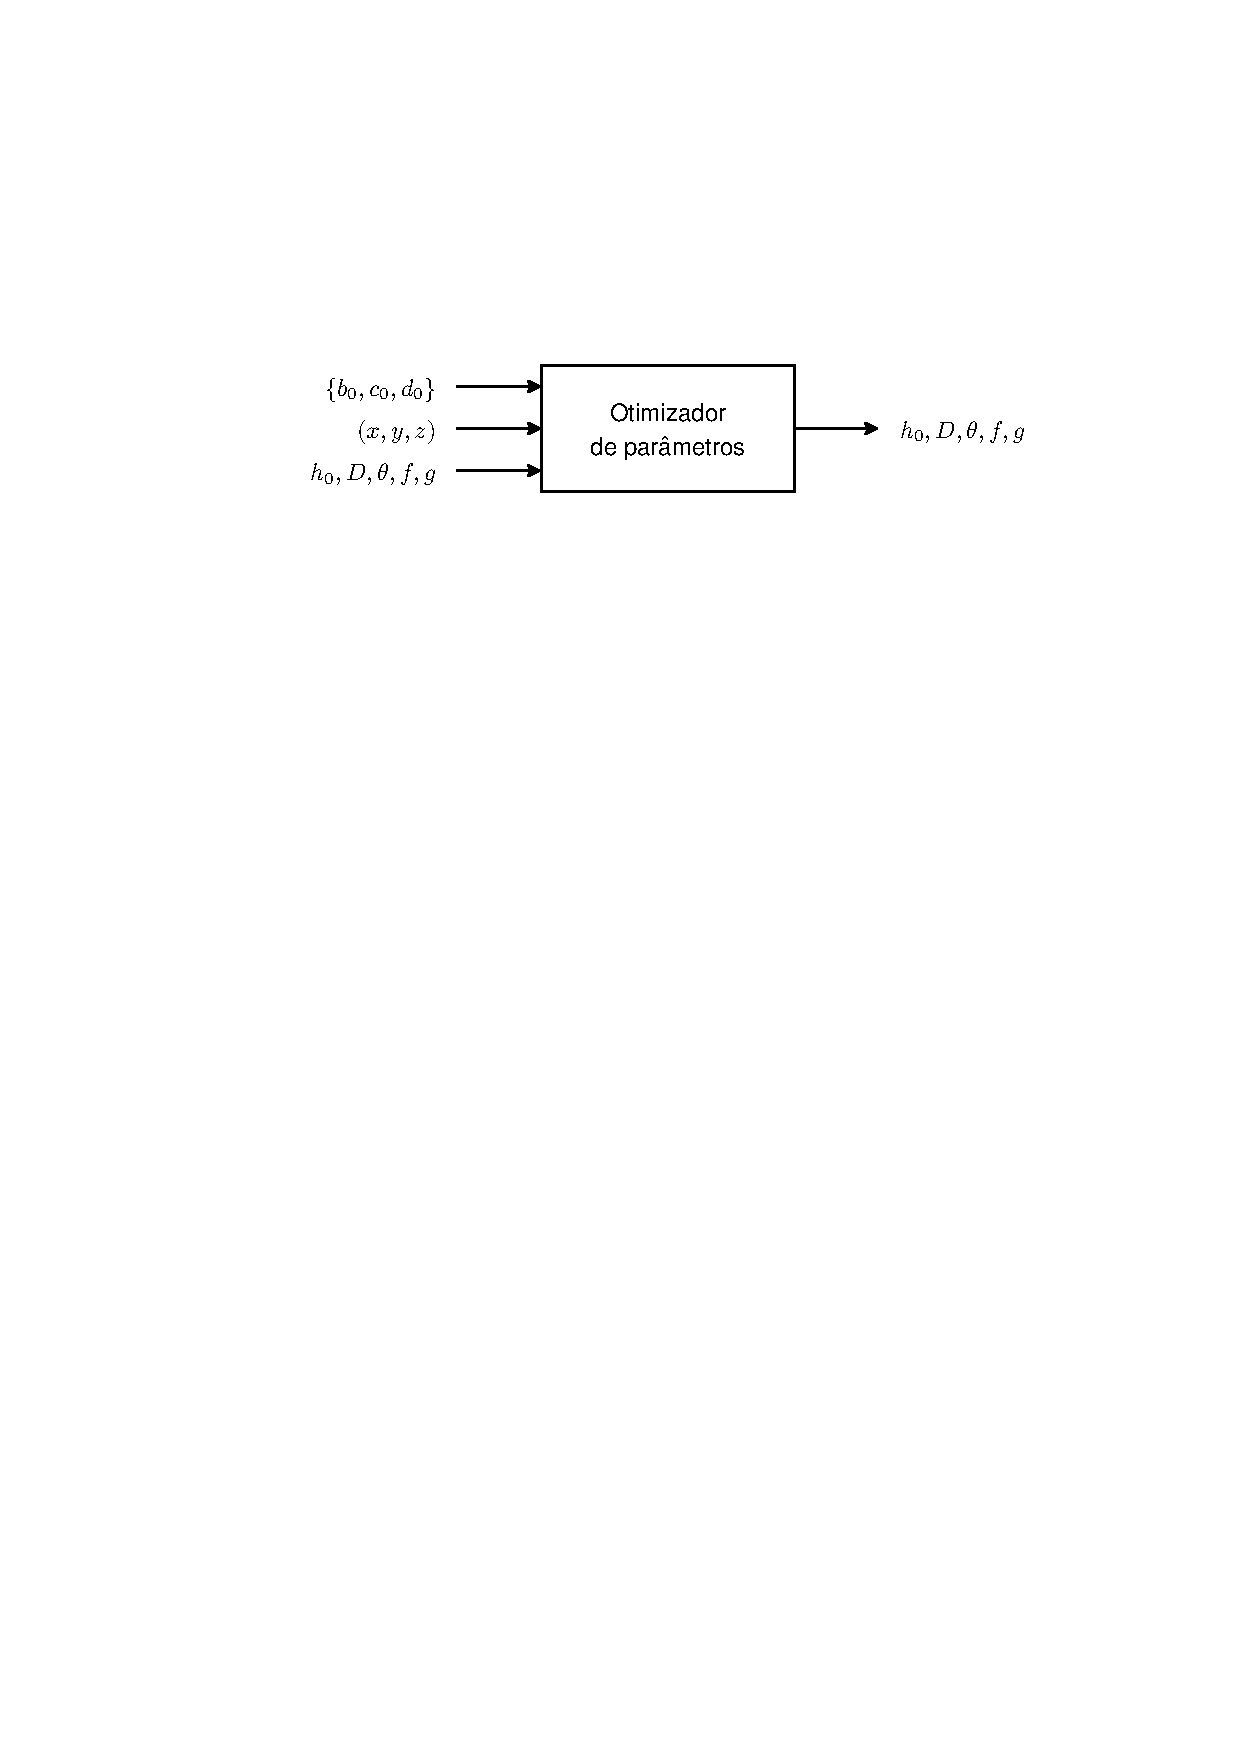
\includegraphics[width=.55\linewidth]{sitema_otimizacao.png}
	\caption{Sitema para otimizar parâmetros}
	\label{sitema_otimizacao}
\end{figure}

Utilizando o software Octave, foi possível desenvolver um algoritmo que fosse capaz de otimizar os dados inseridos manualmente e retornar o melhor valor da medição com o menor erro possível. Baseado nos passos descritos no fluxograma da Figura \ref{identificar parametros}, foi possível realizar essa aproximação dos dados.


\begin{figure}[H]
	\centering
		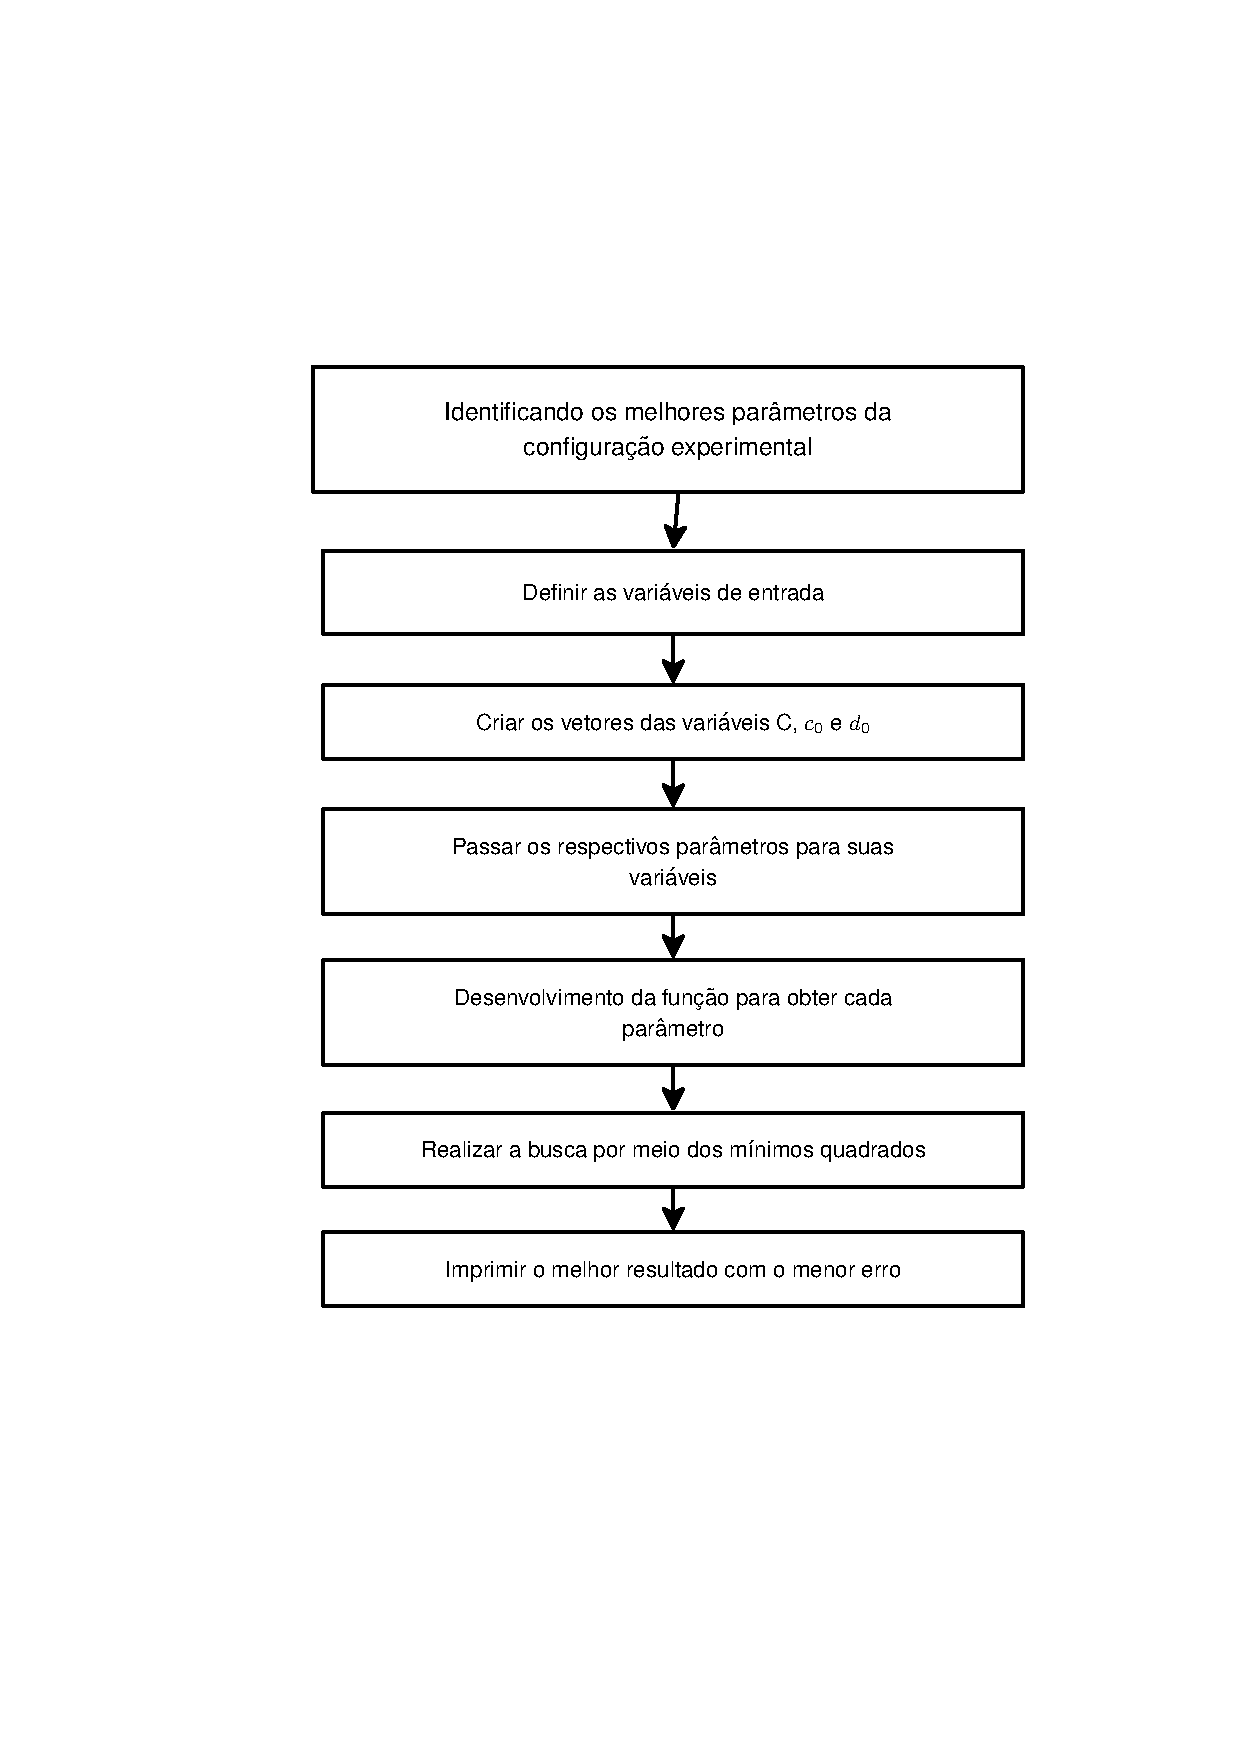
\includegraphics[width=.55\linewidth]{fluxograma_identificar_parametros.png}
	\caption{Fluxograma para identificar parâmetros}
	\label{identificar parametros}
\end{figure}

Para desenvolver o algoritmo de otimização dos parâmetros, primeiro definiram-se os parâmetros do sistema como sendo $h_0$, D, Q, f e g, para receber os dados calculados manualmente. Logo, foi criado um vetor com o propósito de receber os parâmetros de $c_0$ e $d_0$ que foram calculados do primeiro objeto digitalizado, com o objetivo de otimizar e identificar os melhores parâmetros para z.

Uma função para receber todos os dados da geometria foi desenvolvida. Utilizou-se de cálculos matemáticos baseados no método dos mínimos quadrados, pelo qual se procurou encontrar o melhor ajuste para o conjunto de dados medidos manualmente, tentando minimizar a soma dos quadrados das diferenças entre os valores estimados e os dados medidos manualmente; porém, utilizar parâmetros calculados medidos manualmente apresentou respostas com erros.

Para melhorar os parâmetros medidos manualmente, foi necessário oferecer mais parâmetros de entrada ao sistema da Figura \ref{sitema_otimizacao}; porém, desta vez, recebendo como parâmetros de entrada $c_0$, correspondente às linhas projetadas no plano em relação às mesmas linhas em cima do objeto, $d_0$ correspondente à diferença entre o meio da imagem e à linha de referência no plano e à variável z, como a altura real do objeto.

Com o conjunto de parâmetros f, g, $h_0$, $c_0$, $d_0$ calculados manualmente, realizaram-se as interações com base nos três parâmetros de entrada que retornaram ao melhor valor dos parâmetros do sistema, ou seja, oferecendo os parâmetros certos citados acima, o sistema funcionou perfeitamente, Figura \ref{sitema_otimizacao}. Uma variável E foi inserida ao algoritmo para representar o valor do erro estimado entre as interações feitas nos parâmetros no algoritmo. Essa variável representou que quanto menor o erro, melhor a interação realizada.

Para que a otimização desses parâmetros alcançasse seus melhores resultados, foram utilizados no mínimo 5 grupos de $c_0$, $d_0$ e z, que foram oferecidos em blocos/vetor, pois quanto mais amostras de entrada para z, $c_0$ e $d_0$, melhor os ajustes dos parâmetros e com retorno de valores mais favoráveis para $h_0$, D, Q, f e g. 

\subsection{Lógica matemática para otimização dos parâmetros do sistema}

Inserir o texto com as formulas do arquivo enviado


\section{Resultados e Discussões}

Utilizando apenas uma câmera fixada a uma distância de 136 centímetros em relação ao objeto e a uma altura de 75 centímetros da superfície; um projetor multimídia fixado a uma distância de 171 centímetros do objeto a ser analisado e a uma altura de 112 centímetros da superfície; em seguida, foi possível projetar linhas sobre o objeto de estudo e resultar em seu perfil após o processamento das imagens. A Figura \ref{arranjo-experimetal} ilustra a disposição dos equipamentos, bem como suas respectivas medidas.


\section{Conclusões}


Foi possível desenvolver uma configuração experimental baseada no método interferométrico a partir de apenas uma webcam e um projetor multimídia. 


\section*{Referências}

LUKAC, R.; PLATANIOTIS, K. N. Desenvolvimento universal para tubulações de imagem com uma matriz de filtros de cores RGB. Reconhecimento de Padrões , v. 38, n. 11, p. 2208-2212, 2005.
\vspace{.5cm}

RIBEIRO, E.; Correção digital das distorções em imagens provenientes de digitalização tridimensional. 98p. Dissertação (Mestrado em Engenharia de Sistemas) – Universidade Federal de Lavras, 2014. 
\vspace{.5cm}

RIVERA, F. P.; Métodos numéricos: Problemas não lineares e inversos, ISBN:978-65-00-07314-0,1ra ed.,agosto 2020.
\vspace{.5cm}



\end{document}
